\section{Shashlik + Hadron Endcap} \label{section:simulations_shashlik}

\begin{figure}[hbp]
    \centering
    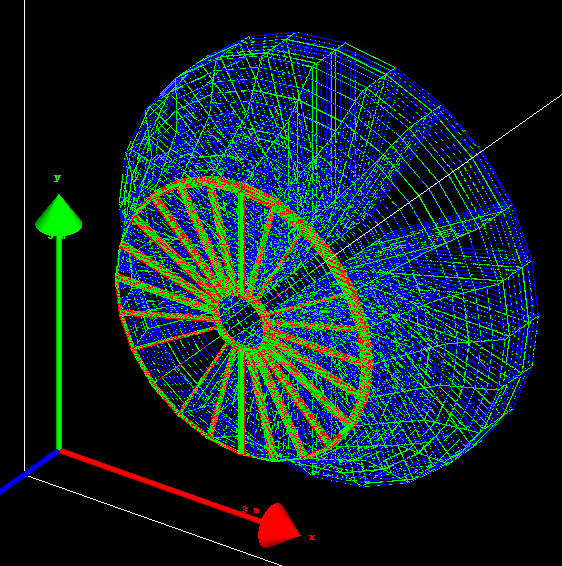
\includegraphics[width=0.9\textwidth]{figures/ch_simulations/shashlik/geometry/Shashlik+HE_Complete_Wire.png}
    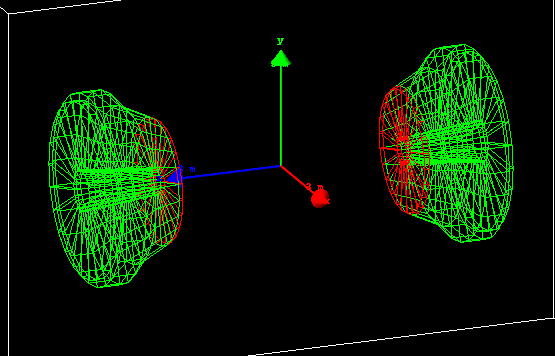
\includegraphics[width=0.9\textwidth]{figures/ch_simulations/shashlik/geometry/SHE_70_20.png}
    \caption{Full CMS Scale Shashlik + HE System (Top/Bottom)}
    \label{fig:higgs_simulations_shashlikexamples}
 \end{figure}

\subsection{Physical Layout}
Shashlik is an Electromagnetic Calorimeter System with the name reflecting its  structure and choice of readout technology. The physical layout is similar to HGC~\ref{section:simulations_hgc}: alternating layers of absorber and active material, however there is no electronics unit sitting on the calorimeter itself. Instead, wave-length shifting fibers go through the whole length of the calorimeter and are responsible for light capture and transmission to the electroncs unit for conversion into analog signal. Full specification of the Shashlik Calorimeter can be summarized as follows:
\begin{itemize}
    \item 25-30 $X_0$ device
    \item No Longitudinal Segmentation
    \item Alternating layers of absorber (W) and active (LYSO) materials.
    \item Active Material used is LYSO plastic scintillator.
\end{itemize}
Hadron Endcap is an active CMS Endcap Calorimeter that is part of the HCAL subsystem. Design principles are similar with respect to Shashlik, however has a different choice of readout technology (described in ~\ref{subsection:higgs_cms_hcal}). Calorimeter specification can be summarized as follows:
\begin{itemize}
    \item $10\lambda$ device
    \item Alternating layers of absorber (Brass) and active (SCSN-81 plastic scintillator) materials
    \item Partial Longitudinal segmentation
\end{itemize}

\subsection{Detector Readout}
For the purpose of simplification, in our simulation we assume perfect light capture and transmission for both Shashlik and Endcap. We also do not model the wave-length shifting fibers or any kind of photodetectors. In other words, we are looking for upper limits of our calorimeter performance. The metric of the system's response we define to be the number of generated photons within the scintillator. Scintillation mechanics is responsible for light generation and G4Scintillation class of Geant4 provides these capabilities via Optical Photons. For the purpose of modeling, Geant4 defines two different types of photons: regular photons, that obey the laws of quantum physics, and optical photons, that follow the laws of geometrical optics. Optical photons do not participate in conservation of energy laws and do not deposit any energy into the scintillator (this fact allows for various optimizations described further).

\subsection{Parametrized Detector Readout}
Typical light yields for a scintillator are in thoughsands of optical photons per 1 MeV of deposited energy into the scintillation material. The exact number is material-dependent and varies substantially. Given that the input particle has energies in the GeV range, the number of optical photons that gets generated goes well above 1M. Tracing all of these photons is a complicated and time-consuming task for Geant's engine. Moreover, given that optical photons can not deposit energy into the material, we can simply ``count and kill them'' right after they've been generated. Therefore, for the purpose of optimizing the time it takes to generate 1 event, we parametrize the response of a schintillator. This procedure allows us to substantially speed up our simulation without degrading the performance.

\subsection{Analysis}
The analysis procedure is identical to the one described for HGC in section~\ref{section:simulations_hgc} and we will not repeat it here. The main differences are in the readout metric (generated photons instead of electron-hole pairs) and the Total Calorimeter Response, which we define to simply be the total number of generated optical photons. Figures~\ref{fig:simulations_shashlik_energyreco},~\ref{fig:simulations_he_energyreco} show the reconstructed energy distributions for Shashlik and HE, respectively. Shashlik and HE are calibrated separately as they constitute isolated parts of a single system. Note this is different with repsect to HGC, where we have calibrated the EM and FH parts together.

\begin{figure}[hbp]
    \centering
    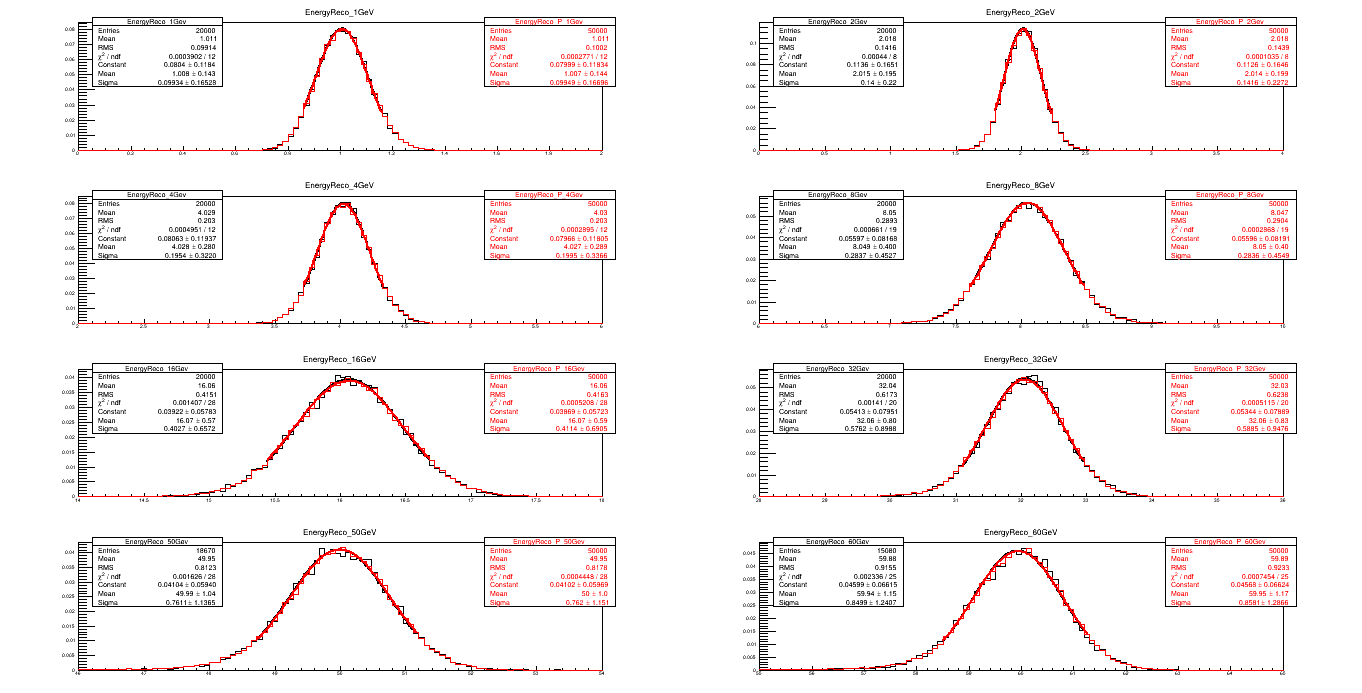
\includegraphics[width=0.95\textwidth]{figures/ch_simulations/shashlik/performance/EnergyRecoDistributions.png}
    \caption{Reconstructed Energy Distributions}
    \label{fig:simulations_shashlik_energyreco}
 \end{figure}

  \begin{figure}[hbp]
    \centering
    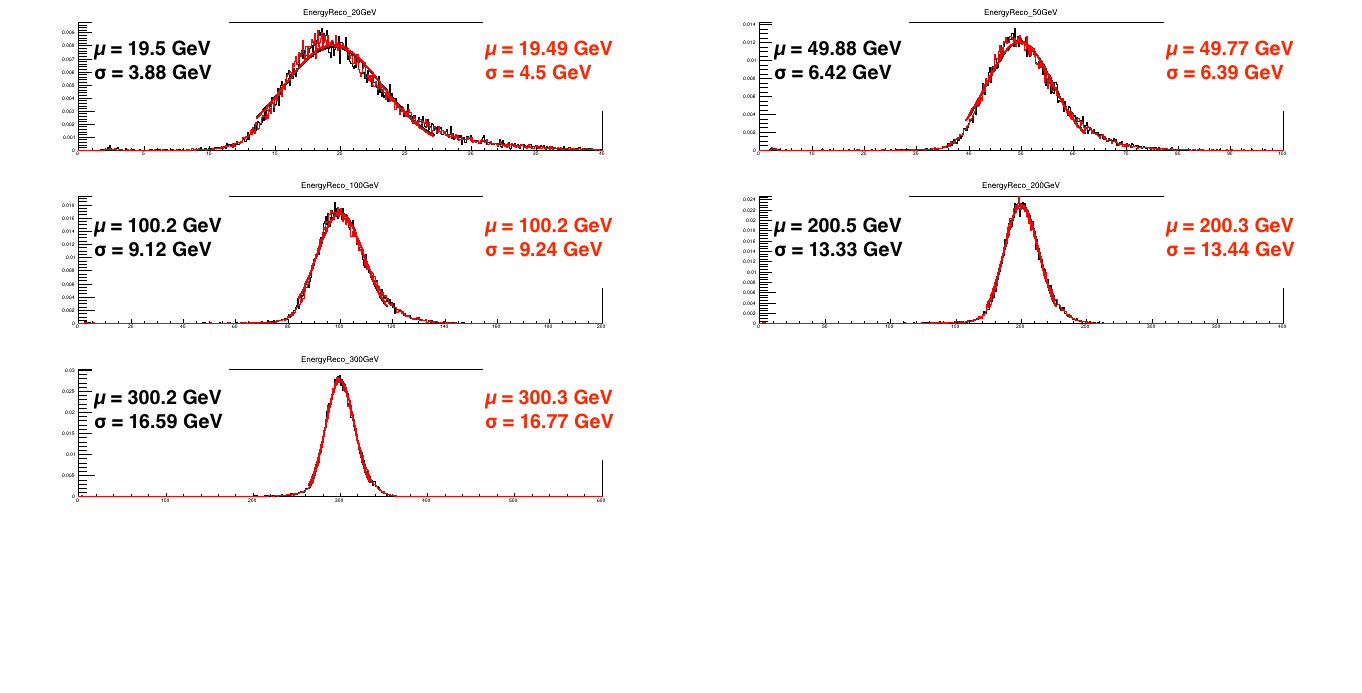
\includegraphics[width=0.95\textwidth]{figures/ch_simulations/he/performance/EnergyRECODistributions.png}
    \caption{Reconstructed Energy Distributions}
    \label{fig:simulations_he_energyreco}
 \end{figure}

 Results for the linearity and energy resolution are provided in figures~\ref{fig:simulations_shashlik_linearityresolution}, ~\ref{fig:simulations_he_linearityresolution}. The differences between the parametrized response and the use of optical photons is negligible.

 \begin{figure}[hbp]
    \centering
    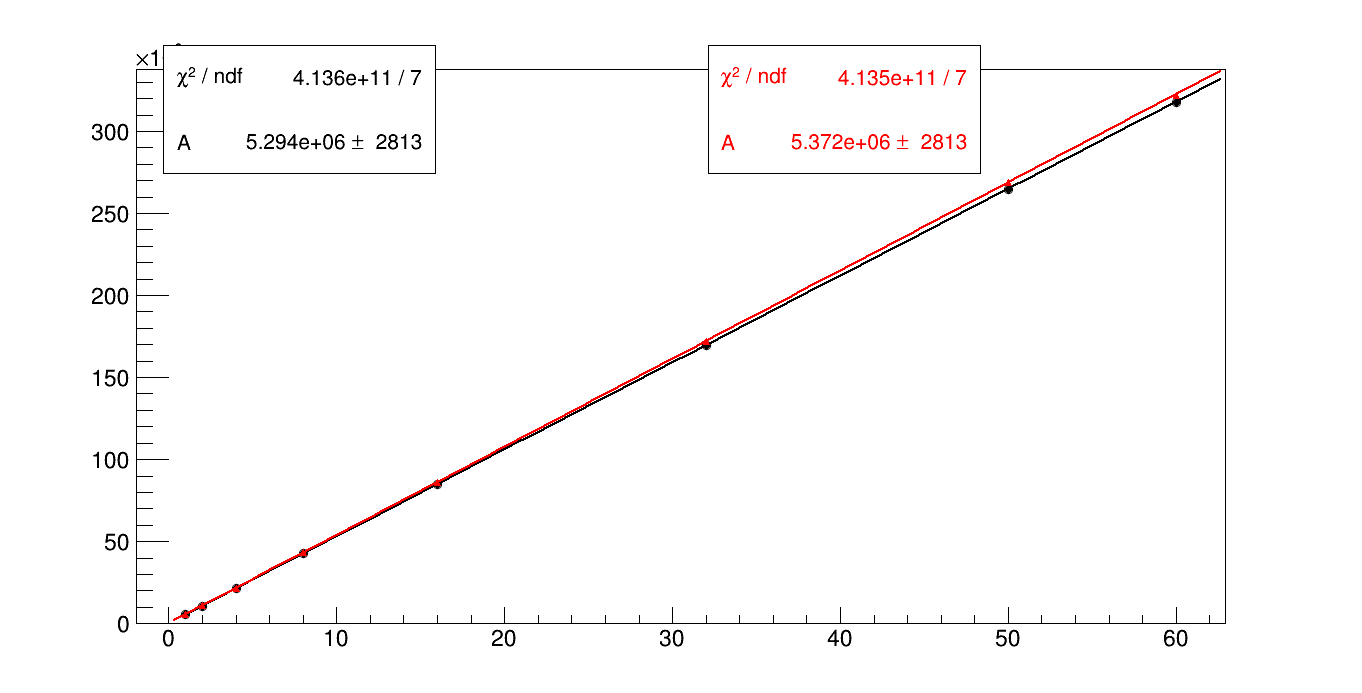
\includegraphics[width=0.9\textwidth]{figures/ch_simulations/shashlik/performance/ResponseVsEnergy.png}
    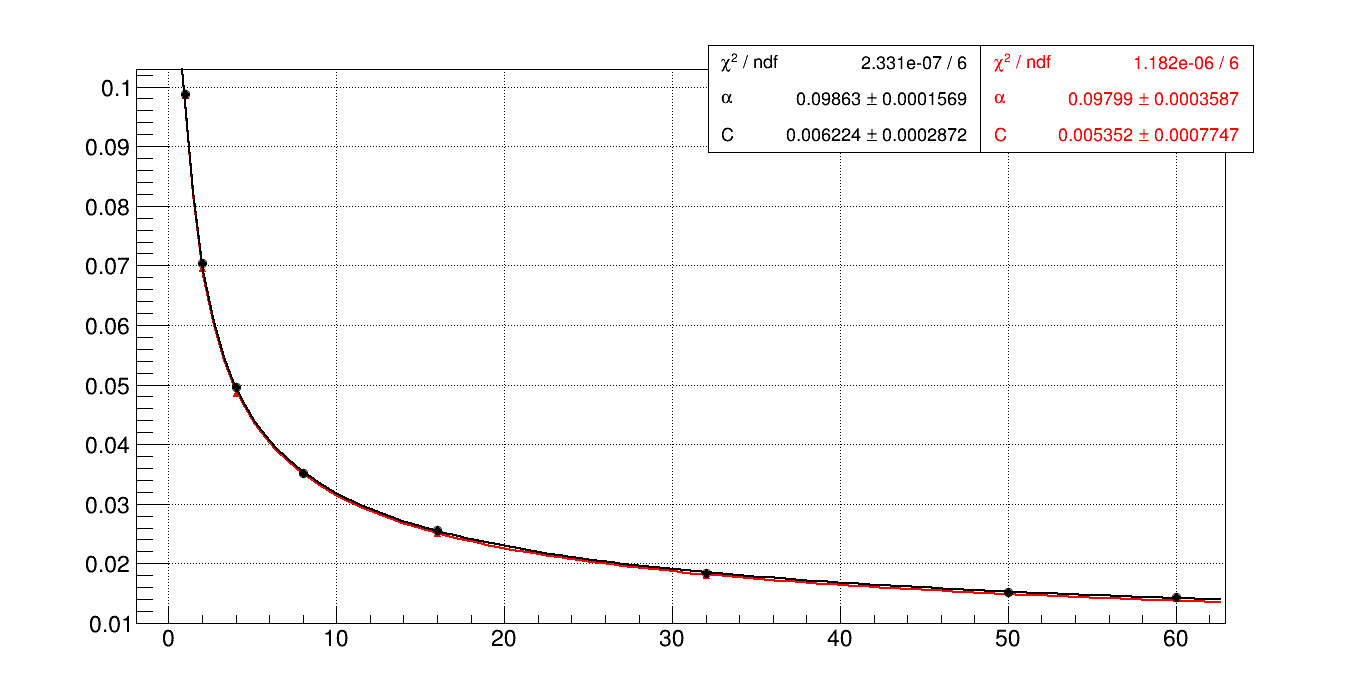
\includegraphics[width=0.9\textwidth]{figures/ch_simulations/shashlik/performance/energyResolution.png}
    \caption{Linearity (Top) and Energy Resolution (Bottom)}
    \label{fig:simulations_shashlik_linearityresolution}
 \end{figure}


 \begin{figure}[hbp]
    \centering
    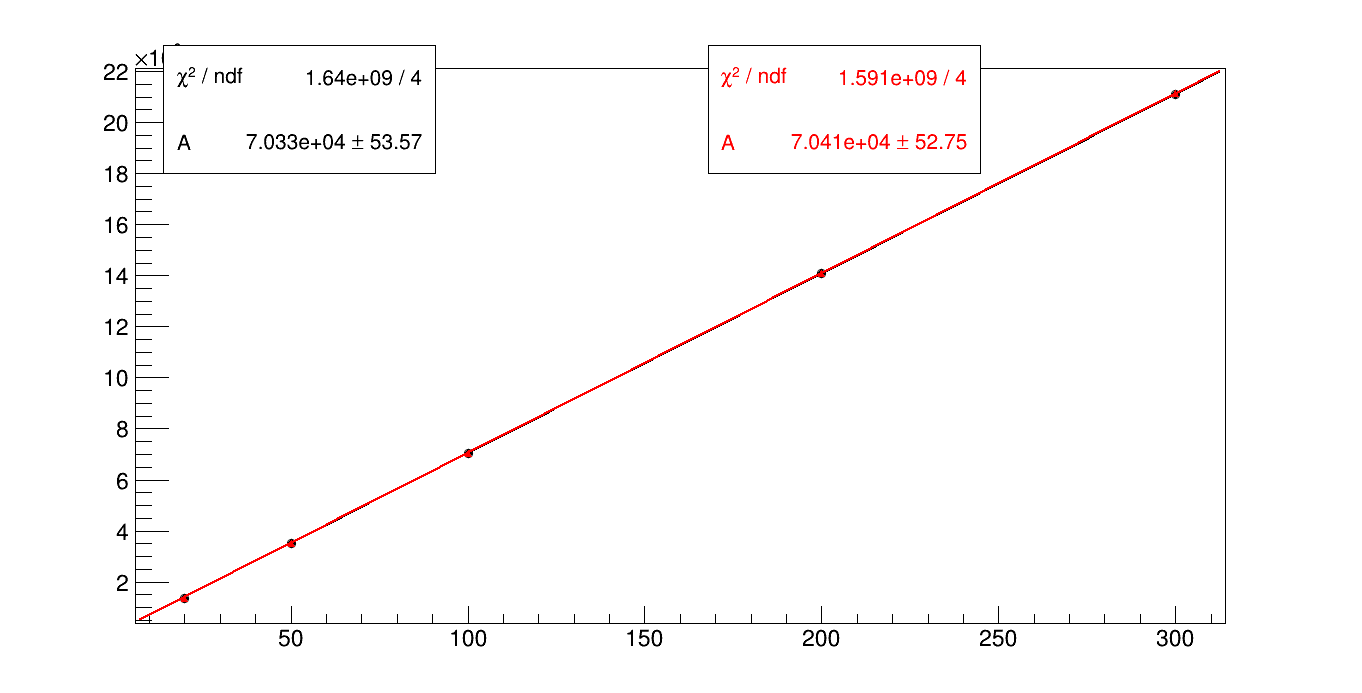
\includegraphics[width=0.9\textwidth]{figures/ch_simulations/he/performance/Linearity.png}
    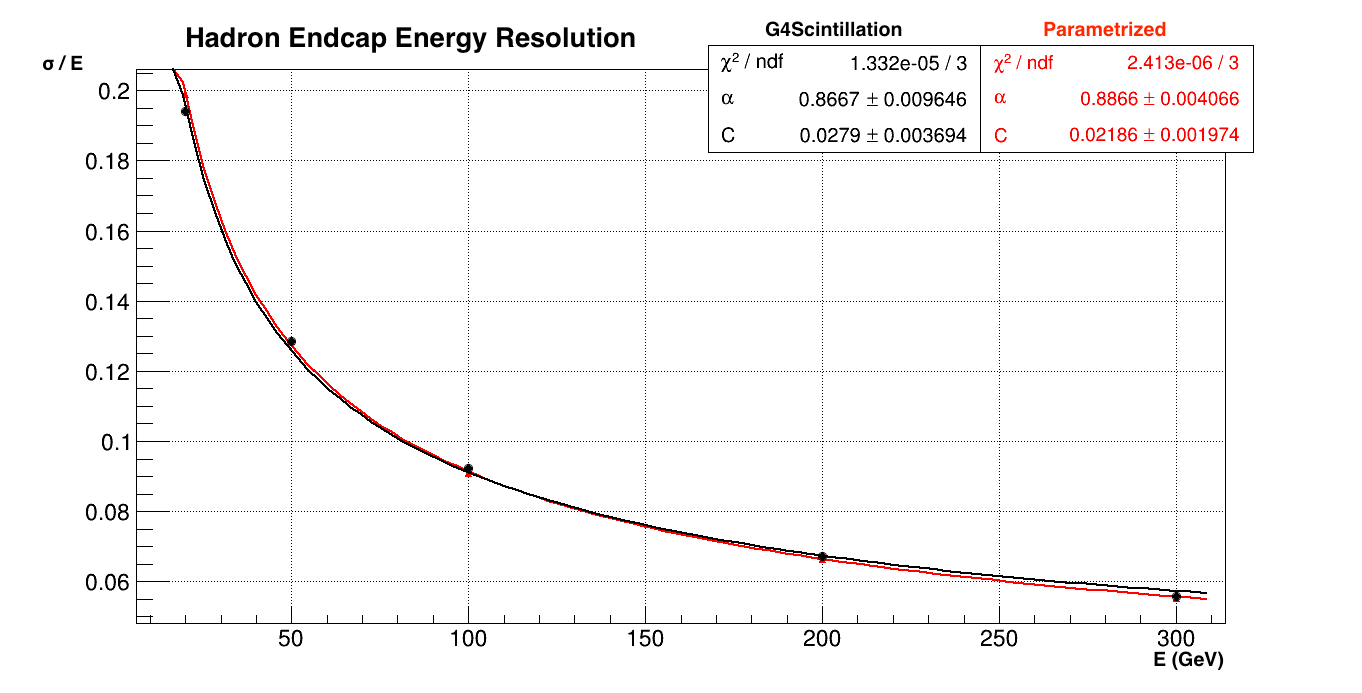
\includegraphics[width=0.9\textwidth]{figures/ch_simulations/he/performance/Resolution.png}
    \caption{Linearity (Top) and Energy Resolution (Bottom)}
    \label{fig:simulations_he_linearityresolution}
 \end{figure}